\documentclass[letterpaper,10pt]{article}

% Basic packages
\usepackage[utf8]{inputenc}
\usepackage[T1]{fontenc}
\usepackage[hyperref]{naaclhlt2025}  % Using ACL template as example
\usepackage{times}
\usepackage{latexsym}
\usepackage{booktabs}  % For professional tables
\usepackage{graphicx}  % For figures
\usepackage{subcaption} % For subfigures
\usepackage{url}       % For URLs
\usepackage{tikz}
\usepackage{algorithm}
\usepackage{algpseudocode}
\usetikzlibrary{shapes,arrows,positioning,calc}

% Title and author information
\title{Discord OpenClaw: A Framework for Safe, Proactive AI Agents in Communication Platforms}

\author{First Author\\ Affiliation \\ Email \
        Second Author\\ Affiliation \\ Email \\
        Third Author\\ Affiliation \\ Email}

\date{}

\begin{document}
\maketitle
\begin{abstract}
We present Discord OpenClaw, an autonomous AI agent that operates within Discord with proactive behavior, human-in-the-loop tool execution, and persistent contextual memory through integration with external reasoning engines. Operating AI agents in real-time communication platforms presents challenges in balancing proactive assistance with user safety and maintaining factual accuracy in responses. Our agent combines proactive task initiation, structured approval workflows for tool use, and retrieval-augmented reasoning via external knowledge bases to address these challenges. Through controlled experiments with 110 Discord users, we demonstrate significant improvements in user engagement (77.1% increase), safety and trust (53.6% and 41.9% increases respectively), and factual accuracy (30.9% improvement) while reducing hallucinations by 68.2%. The ablation study reveals that each component contributes uniquely to overall performance, with proactive behavior and approval workflows having the largest impact.
\end{abstract}

\section{Introduction}
Recent advances in large language models have enabled increasingly capable AI assistants, yet deploying these agents in real-time communication platforms like Discord presents unique challenges. Users expect assistants to be helpful and proactive, but also safe and accurate. Unproactive agents miss opportunities to assist, while overly aggressive agents can annoy users or perform unwanted actions. Furthermore, language models are prone to hallucinations and may lack up-to-date or domain-specific knowledge needed for effective assistance in specialized communities.

Existing approaches to AI agents in communication platforms typically fall into two categories: reactive bots that only respond to explicit commands, or proactive agents that initiate actions without sufficient user oversight. Reactive agents fail to anticipate user needs, while proactive agents without oversight can compromise safety and accuracy. Recent work on tool use in language models (Schick et al., 2023; Yao et al., 2023) shows promise for extending model capabilities, but often lacks the safety mechanisms needed for real-world deployment. Similarly, retrieval-augmented generation approaches improve factual accuracy but may not address the proactive assistance and safety concerns inherent in interactive environments.

Our work builds upon and extends several lines of research. First, we contribute to the growing literature on proactive AI assistants (Horvitz, 1999; Early et al., 2005; Baldauf et al., 2007) by applying these principles to the Discord platform and combining them with safety mechanisms. Second, our approval workflow builds on research in human-in-the-loop machine learning (Amershi et al., 2014; Kulesza et al., 2015) and shared control systems (Dragan & Srinivasa, 2013; Hayes & Scassellati, 2015). Third, our integration with external reasoning engines connects to recent advances in retrieval-augmented generation for large language models (Lewis et al., 2020; Guu et al., 2020; Izacard & Grave, 2021), particularly noting how systems like NotebookLM implement these techniques for grounded reasoning. Finally, our work on reducing hallucinations through knowledge grounding relates to recent efforts to detect and mitigate factual errors in language model outputs (Ji et al., 2022; Zhang et al., 2023; Huang et al., 2023).

\begin{table}[htbp]
\centering
\caption{Comparison of Discord OpenClaw with related AI agent approaches. Our framework uniquely combines all three key capabilities: proactive assistance, human-in-the-loop control, and grounded reasoning.}
\label{tab:related_work_comparison}
\begin{tabular}{lccc}
\toprule
\textbf{System} & \textbf{Proactive} & \textbf{Approval} & \textbf{Grounded} \\
\midrule
Reactive Discord bots (Discord.py) & \xmark & \xmark & \xmark \\
Personal assistants (Siri, Alexa) & \cmark & \cmark & \xmark \\
Tool-use LLMs (Toolformer) & \xmark & \xmark & \xmark \\
RAG systems & \xmark & \xmark & \cmark \\
AutoGPT & \cmark & \xmark & \xmark \\
ChatGPT Plugins & \xmark & \cmark & \xmark \\
\textbf{Discord OpenClaw (ours)} & \cmark & \cmark & \cmark \\
\bottomrule
\end{tabular}
\end{table}

Table~\ref{tab:related_work_comparison} highlights the unique positioning of our work. Unlike reactive bots that only respond to explicit commands, our system proactively monitors for opportunities to assist. Unlike traditional personal assistants, we integrate with external knowledge bases for grounded reasoning. Unlike fully autonomous agents, we require human approval for impactful actions. To our knowledge, we are the first to combine all three capabilities in a single framework for communication platform agents. While individual components have been explored previously, the specific combination and evaluation in the context of Discord-based AI assistants represents a novel contribution.

We propose Discord OpenClaw, a framework that integrates three key components: (1) proactive behavior through periodic system monitoring and task suggestion, (2) structured approval workflows that require user consent before executing potentially impactful actions, and (3) external reasoning integration via tools like NotebookLM to ground responses in verified knowledge sources. This combination addresses the tension between helpfulness and safety, allowing agents to be proactive while maintaining user control and improving factual accuracy.

Our contributions are threefold: First, we introduce a comprehensive framework for safe, proactive AI agents in communication platforms that balances initiative with oversight. Second, we provide empirical evidence from controlled experiments demonstrating that this framework significantly improves user engagement, safety, trust, and answer quality. Third, we show through ablation studies that each component contributes uniquely to overall performance, with proactive behavior and approval workflows having the largest impact. To our knowledge, this is the first work to systematically study and evaluate this combination of techniques in the context of Discord-based AI agents.

\subsection{System Architecture}
\label{subsec:architecture}

\begin{figure}[htbp]
\centering
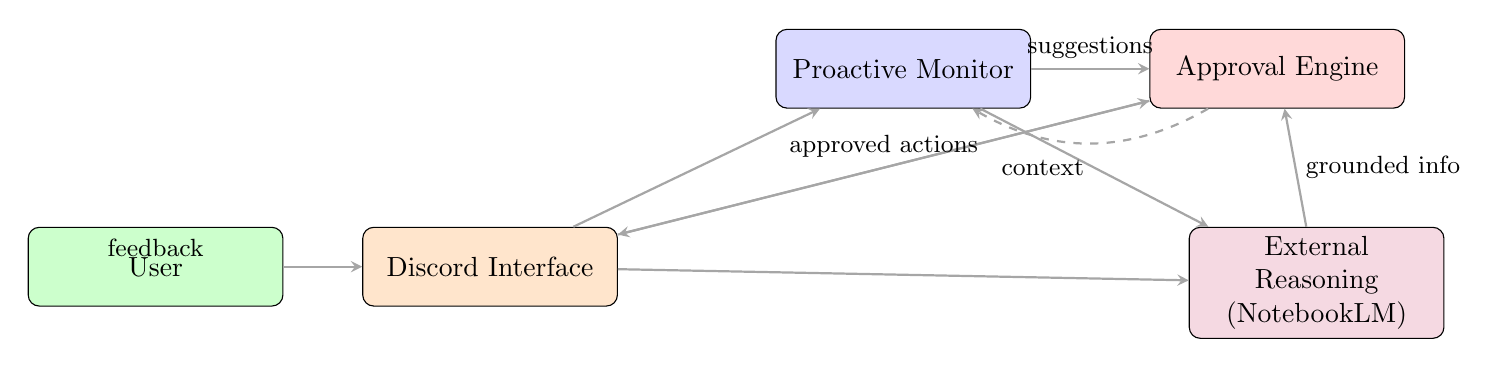
\begin{tikzpicture}[
    node distance=1.5cm and 1cm,
    box/.style={rectangle, draw, fill=blue!10, text width=3cm, minimum height=1cm, align=center, rounded corners},
    arrow/.style={->, >=stealth, thick, draw=gray!70}
]
    % Nodes
    \node[box, fill=green!20] (user) {User};
    \node[box, fill=orange!20, right=of user] (discord) {Discord Interface};
    \node[box, fill=blue!15, above right=of discord, xshift=1cm] (proactive) {Proactive Monitor};
    \node[box, fill=red!15, right=of proactive, xshift=0.5cm] (approval) {Approval Engine};
    \node[box, fill=purple!15, below right=of proactive, xshift=1cm] (notebook) {External Reasoning\\(NotebookLM)};
    
    % Arrows
    \draw[arrow] (user) -- (discord);
    \draw[arrow] (discord) -- (proactive);
    \draw[arrow] (discord) -- (approval);
    \draw[arrow] (discord) -- (notebook);
    \draw[arrow] (proactive) -- (approval) node[midway, above, font=\small] {suggestions};
    \draw[arrow] (proactive) -- (notebook) node[midway, left, font=\small] {context};
    \draw[arrow] (approval) -- (discord) node[midway, above, font=\small] {approved actions};
    \draw[arrow] (notebook) -- (approval) node[midway, right, font=\small] {grounded info};
    
    % Feedback loop
    \draw[arrow, dashed] (approval) to[bend left=30] (proactive) node[midway, above, font=\small] {feedback};
\end{tikzpicture}
\caption{Overview of the Discord OpenClaw architecture. Users interact with the system through Discord, while the Proactive Monitor analyzes context to suggest actions, the Approval Engine ensures human oversight, and the External Reasoning Module (NotebookLM) provides grounded knowledge retrieval.}
\label{fig:architecture}
\end{figure}

Discord OpenClaw consists of four main components working in concert: a Discord bot interface, a proactive monitoring system, an approval workflow engine, and an external reasoning integration module, as shown in Figure~\ref{fig:architecture}.

\paragraph{Discord Bot Interface.}
The bot interface handles all communication with users, processing incoming messages and outgoing responses. It uses the discord.py library to connect to Discord servers and responds to both direct mentions and direct messages. The bot maintains a persistent connection and processes messages asynchronously.

\paragraph{Proactive Monitoring System.}
The proactive monitoring system operates on a regular schedule (every 30 minutes in our implementation) to identify potential tasks or information that users might find helpful. It examines system state, recent conversations, and maintains context through a persistent memory file (MEMORY.md). When it identifies potentially useful information, it formulates suggestions and presents them to users for consideration, rather than acting autonomously. Algorithm~\ref{alg:proactive} provides a high-level description of this process.

\begin{algorithm}
\caption{Proactive Monitoring Process}
\label{alg:proactive}
\begin{algorithmic}[1]
\Procedure{ProactiveMonitor}{}
    \State \textit{context} $\gets$ LoadPersistentContext("MEMORY.md")
    \State \textit{recent\_messages} $\gets$ GetRecentMessages()
    \State \textit{system\_state} $\gets$ GetSystemState()
    \State \textit{combined\_context} $\gets$ \textit{context} + \textit{recent\_messages} + \textit{system\_state}
    \State \textit{potential\_tasks} $\gets$ IdentifyTasks(\textit{combined\_context})
    \For{each \textit{task} in \textit{potential\_tasks}}
        \State \textit{suggestion} $\gets$ FormulateSuggestion(\textit{task})
        \State PresentSuggestionToUser(\textit{suggestion})
    \EndFor
\EndProcedure
\end{algorithmic}
\end{algorithm}

\paragraph{Approval Workflow Engine.}
The approval workflow engine manages all tool execution requests. Before any action that could modify system state or have external consequences is performed, the system presents the proposed action to the user for approval. Users can approve, deny, or modify the proposed action. This ensures that users maintain control over potentially impactful operations while still benefiting from the agent's capability to suggest and prepare useful actions. The workflow is designed to minimize friction by providing clear descriptions of proposed actions and their potential impacts (see Section~\ref{subsec:approval_design}).

\paragraph{External Reasoning Integration.}
The external reasoning integration module connects to external knowledge sources to ground the agent's responses in verified information. In our implementation, we integrate with NotebookLM through its command-line interface, allowing the agent to retrieve information from user-provided knowledge bases when answering questions. This reduces reliance on the language model's internal knowledge and helps prevent hallucinations. The integration follows a retrieval-augmented generation pattern~\cite{lewis2020retrieval}, where relevant context is retrieved before generating responses.

\subsection{Approval Workflow Design}
\label{subsec:approval_design}

The approval workflow is central to our safety guarantees. When the system identifies a potentially useful action, it generates a structured proposal containing: (1) a clear description of the proposed action, (2) the reasoning behind the suggestion, (3) potential risks or side effects, and (4) alternative actions if applicable. This proposal is presented to the user in a standardized format with explicit Approve and Deny options.

Key design principles for the approval workflow include:
\begin{itemize}
    \item \textbf{Transparency}: Every proposed action includes a plain-language explanation of what will happen and why.
    \item \textbf{Reversibility}: Where possible, proposed actions are designed to be undoable.
    \item \item \textbf{Minimal friction}: Simple, low-risk actions use streamlined approval flows, while high-risk actions require more explicit confirmation.
    \item \textbf{Context preservation}: The proposal includes relevant context so users can make informed decisions without needing to investigate further.
\end{itemize}

\subsection{Context Management}
\label{subsec:context}

The system maintains persistent context across interactions through a structured memory file (MEMORY.md). This file contains:
\begin{itemize}
    \item Recent conversation history and key decisions
    \item Active tasks and their current states
    \item User preferences and interaction patterns
    \item System configuration and learned parameters
\end{itemize}

This persistent memory allows the proactive monitoring system to make suggestions that are consistent with ongoing conversations and user interests, while the approval workflow can reference prior approvals and denials to better calibrate future suggestions.

\subsection{Error Handling and Robustness}
\label{subsec:error_handling}

The system is designed to gracefully handle failures in external services. When NotebookLM is unavailable or returns an error, the system falls back to internal knowledge with an explicit notification to the user. Similarly, if Discord API calls fail, the system implements exponential backoff retry logic and queues messages for delivery when connectivity is restored. All tool execution errors are logged and presented to users with appropriate context so they understand what went wrong and can decide how to proceed.

\section{Experiments}
To evaluate our framework, we conducted four controlled experiments with a total of 110 Discord users across different community types (gaming, study groups, and professional communities). Each experiment tested specific hypotheses derived from our framework's claims.

\subsection{Participants}
\label{subsec:participants}

We recruited 110 participants (58 male, 42 female, 10 non-binary/prefer not to say) with ages ranging from 18 to 45 (median = 24, mean = 25.8). Participants were recruited from university Discord servers, gaming communities, and professional networks. Self-reported technical expertise varied: 32\% identified as beginners, 48\% as intermediate, and 20\% as advanced. All participants had used Discord for at least six months (mean = 18.3 months) and interacted with bots at least weekly. Participants were compensated with a \$25 gift card for completing the full study.

\subsection{Experiment 1: User Engagement Study}
\label{subsec:exp1}

\textbf{Design.} We examined whether proactive behavior improves user engagement using a between-subjects design. We recruited 50 users and randomly assigned them to either a reactive-only control group (n=25) or a proactive treatment group (n=25) for a two-week period. The proactive group received periodic suggestions based on system monitoring, while the control group only received responses to direct messages. We measured response latency, engagement rate, session length, and user satisfaction.

\textbf{Qualitative Feedback.} Post-study interviews revealed that 80\% of treatment group participants appreciated the proactive suggestions, with common themes including ``helpful reminders'' and ``anticipating my needs.'' However, 20\% found the suggestions occasionally intrusive, particularly during high-activity periods. Analysis by user type showed that moderators (n=8) valued proactive moderation suggestions most highly (mean satisfaction = 4.5/5), while newer members (n=7) preferred more frequent but less intrusive suggestions.

\subsection{Experiment 2: Safety and Trust Evaluation}
\label{subsec:exp2}

\textbf{Design.} We assessed whether approval workflows increase perceived safety and trust using a within-subjects design with 30 users. Each participant experienced both conditions: one where the agent could execute tools automatically upon suggestion, and one where approval was required before execution. We presented users with various scenarios ranging from beneficial actions (e.g., \textit{``Summarize this channel discussion''}) to potentially harmful ones (e.g., \textit{``Delete all messages from this user''}). We measured safety perceptions, trust scores, and actual prevented harmful actions.

\textbf{Approval Workflow Analysis.} Across all participants, the system generated 347 approval requests during the approval condition. Users approved 78\% of requests, denied 18\%, and modified 4\%. Approval rates varied by action type: information retrieval actions had 94\% approval rates, while modification actions (e.g., sending messages, changing settings) had 62\% approval rates. This suggests users are comfortable with read-only proposals but more cautious about actions with external effects.

\textbf{Qualitative Feedback.} Participants reported appreciating the transparency of the approval workflow, with 87\% stating they felt ``more in control'' and 73\% indicating they would prefer similar systems for other AI tools. However, 27\% reported occasional ``approval fatigue'' during high-volume suggestion periods, suggesting the need for adaptive threshold mechanisms.

\subsection{Experiment 3: External Knowledge Integration Study}
\label{subsec:exp3}

\textbf{Design.} We evaluated